% !TEX root = ../../main.tex
\subsection{Kolmogorov backward equation}

So far with the Fokker-Planck equation we have been able to ask questions about
the entire distribution of allele frequencies accounting for the interplay of
different evolutionary forces simultaneously. Another interesting set of
questions has to do with asking what is the probability of the population
reaching a specific subset of states in a time $s > t$ given the current state
of the population $f(t)$. To be more specific we can ask what is the
probability of fixing an allele in a population as a function of its selective
advantage. For this kind of questions we use the so-called Kolmogorov-backward
equation. The name comes from the fact that compared to the forward equation,
i.e. the Fokker-Planck equation we derived in the previous section, we need to
integrate backwards in time.

The main difference between the forward and the backward equation has to do
with the emphasis on either the initial condition or the current state. As we
showed in \secref{sec_master_eq} the master equation is a statement about the
time evolution of the transition probability $P(f, t \mid f', t')$ for $t' \leq
t$. Let us set $f' \equiv f_o$, $t' \equiv t_o$ to be the initial conditions of
the random walker in allele frequency space. We then ask about the probability
of being at frequency $f$ at time $t$, i.e. $P(f, t + \Dt \mid f_o, t_o)$. This
probability is related to all of the possible paths that the variable $f$ can
take from the initial value $f_o$ at time $t_o$ to the value $f$ as shown
schematically in \fref{fig_03_05_01}.

\begin{figure}[h!]
	\centering 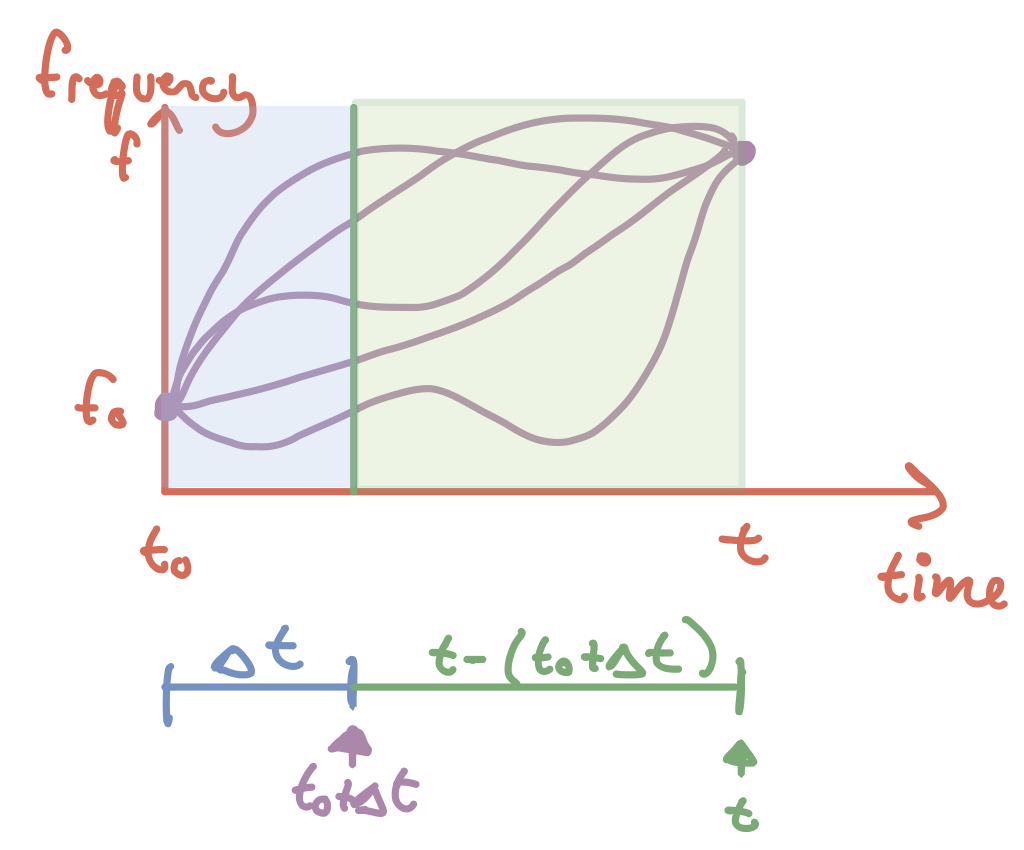
\includegraphics[width=0.5\textwidth]
  {../fig/classic_diffusion/03_05_01_schematic_reverse.png}
	\caption{\textbf{Schematic depiction of paths from $f_o$ to $f$}. The
	diagram shows schematically different paths that the allele frequency can
	take from an initial condition $f_o$ to a final point $f$ over a time $t$.
	The time is arbitrarily split into two intervals $[t_o, t_o + \Dt]$ shaded
	in blue and $[t_o + \Dt, t]$ shaded in green.}
  \label{fig_03_05_01}
\end{figure}

\subsubsection{Derivation of the Kolmogorov backward equation}

To derive the backward equation we can arbitrarily split the time interval in
two intervals $[t_o, t_o + \Dt]$ and $[t_o + \Dt, t]$. With this we can then
write down the Chapman-Kolmogorov equation that we stated in
\secref{sec_chapman_kolmogorov} as
\begin{equation}
  P(f, t \mid f_o, t_o) = \int_{-f_o}^{1 - f_o} dr \;
  P(f, t \mid f_o + r, t_o + \Dt)
  P(f_o + r, t_o + \Dt \mid f_o, t_o),
\end{equation}
where the limits of the integral on the right hand side were set such that the
quantity $f_o + r$ could cover the entire domain $[0, 1]$. For $\Dt$ very
small, specifically $\Dt \ll |t - t_o|$ we can write down the transition matrix
as we did for \eref{eq_transition_short_time}, obtaining
\begin{equation}
	P(f_o + r, t_o + \Dt \mid f_o, t_o) =
	\delta(r) \left[
	1 - a^{(0)}(f_o, t_o) \Dt
	\right] +
	\phi_{t_o}(f_o; r) \Dt,
\end{equation}
where $\phi_{t_o}(f_o; r) \Dt$ is the probability of taking a jumpt of size $r$
on a time window $\Dt$ given the initial position $f_o$ In this case the
$\delta$-function $\delta(r)$ is equal to one only when the jump $r$ is zero.
Notice that compared to the derivation of the forward equation where we first
wrote the corresponding master equation, here we start directly from the
transition distribution as a function of the jump size $r$. Substituting this
into the Chapman-Kolmogorov equation gives
\begin{equation}
	P(f, t \mid f_o, t_o) = \int_{-f_o}^{1 - f_o} dr\;
	P(f, t \mid f_o + r, t_o + \Dt)
	\left[
	\delta(r) \left( 1 - a^{(0)}(f_o, t_o) \Dt \right) +
	\phi_{t_o}(f_o; r) \Dt
	\right].
\end{equation}
If we distribute the integral and evaluate it over the delta function we obtain
\begin{equation}
	\begin{split}
		P(f, t \mid f_o, t_o) = P(f, t \mid f_o, t_o + \Dt)
		\left[
		1 - a^{(0)}(f_o, t_o)\Dt
		\right]\\ +
		\int_{-f_o}^{1 - f_o} dr\; P(f, t \mid f_o + r, t_o + \Dt)
		\phi_{t_o}(f_o; r) \Dt.
	\end{split}
	\label{eq_chap_kol_delta_eval_backwards}
\end{equation}
In \eref{eq_a0} we showed that $a^{(0)}(f_o, t_o)\Dt$ is the probability of
transitioning from $f_o$ to anywhere else. This is equivalent to writing
\begin{equation}
	a^{(0)}(f_o, t_o) \Dt \equiv \int_{-f_o}^{1 - f_o} dr \;
	\phi_{t_o}(f_o; r) \Dt.
\end{equation}
Substituting this result into \eref{eq_chap_kol_delta_eval_backwards} and
rearranging terms gives
\begin{equation}
	\begin{split}
	{P(f, t \mid f_o, t_o) - P(f, t \mid f_o, t_o + \Dt) \over \Dt} =
	- P(f, t \mid f_o, t_o + \Dt) \int_{-f_o}^{1 - f_o} dr \;
	\phi_{t_o}(f_o; r)\\
	+ \int_{-f_o}^{1 - f_o} dr \;
	P(f, t \mid f_o + r, t_o + \Dt) \phi_{t_o}(f_o; r).
	\end{split}
	\label{eq_almost_kolmogorov_backwards}
\end{equation}
If we assume our stochastic process is stationary (See
\secref{sec_stationary_process}), a perfectly reasonable assumption for a
fixed fitness landscape, it follows that
\begin{equation}
	 P(f, t + \tau \mid f_o, t_o + \tau) = P(f, t \mid f_o, t_o),
\end{equation}
for any $\tau$. In other words, for our stationary stochastic process what
matters is the time interval that happens between events rather than the actual
time. Using this we can then write the first term on the left-hand side of
\eref{eq_almost_kolmogorov_backwards} as
\begin{equation}
	P(f, t \mid f_o, t_o) = P(f, t + \Dt \mid f_o, t_o + \Dt).
\end{equation}
Using this time shift and taking the limit when $\Dt \rightarrow 0$ gives for
the left-hand side of \eref{eq_almost_kolmogorov_backwards}
\begin{equation}
	\lim_{\Dt \rightarrow 0} {P(f, t + \Dt \mid f_o, t_o + \Dt) -
	P(f, t \mid f_o, t_o + \Dt) \over \Dt} =
	\ddt{P(f, t \mid f_o, t_o)}.
\end{equation}
Using this for \eref{eq_almost_kolmogorov_backwards} results in
\begin{equation}
	\ddt{P(f, t \mid f_o, t_o)} =
	- P(f, t \mid f_o, t_o) \int_{- f_o}^{1 - f_o} dr \; \phi_{t_o}(f_o; r)
	+ \int_{- f_o}^{f_o} dr \; P(f, t \mid f_o + r, t_o) \phi_{t_o}(f_o; r).
\end{equation}
Notice we already took the limit $\Dt \rightarrow 0$ on both sides. We now
expand the second term on the right-hand side to obtain an analogous
Kramers-Moyal expansion for the Kolmogorov reverse equation. This is analogous
in the sense that we are not expanding a master equation as we did for the
forward equation. Also for this case we expand around the initial condition
$f_o$ rather than the final position $f$. Since the transition probability
$\phi_{t_o}(f_o; r)$ does not have a term $f_o + r$ it does not take part of
this expansion. Therefore we obtain
\begin{equation}
	\ddt{P(f, t \mid f_o, t_o)} =
	- P(f, t \mid f_o, t_o) \int_{- f_o}^{1 - f_o} dr \; \phi_{t_o}(f_o; r)
	+ \int_{-f_o}^{1 - f_o} dr\; \sum_{k=0}^{\infty} {1 \over k!}
	{\partial^k \over \partial f_o^k} P(f, t \mid f_o, t_o) r^k
	\phi_{t_o}(f_o; r).
\end{equation}
For this expansion we do not have issues with the integration limits. This
again happens because we are not expanding the master equation as we did for
the forward equation. The zero$\tth$ order term in the expansion cancels with
the first term on the right-hand side, obtaining
\begin{equation}
	\ddt{P(f, t \mid f_o, t_o)} =
	\sum_{k = 1}^{\infty} {1 \over k!} {\partial^k \over \partial f_o^k}
	P(f, t \mid f_o, t_o) \int_{-f_o}^{1 - f_o} dr\; \phi_{t_o}(f_o; r) r^k.
\end{equation}
We can again define the moments of the jump distribution $\phi_{t_o}(f_o; r)$
as
\begin{equation}
	a^{(k)}(f_o, t_o) \equiv \int_{-f_o}^{1 - f_o} dr \;
	r^k \phi_{t_o}(f_o; r).
\end{equation}
Using this we obtain the  expansion for the Kolmogorov backward equation
\begin{equation}
	\ddt{P(f, t \mid f_o, t_o)} =
	\sum_{k = 1}^{\infty} {1 \over k!} {\partial^k \over \partial f_o^k}
	P(f, t \mid f_o, t_o) a^{(k)}(f_o, t_o).
\end{equation}
Just as with the forward equation we can truncate the expansion up to second
order. Furthermore we define the first moments to be the mean jump size
\begin{equation}
	M(f_o) = \int_{-f_o}^{1 - f_o} dr \; r \phi_{t_o}(f_o; r).
\end{equation}
For small $M(f_o)$ we approximate the second moment as the variance
\begin{equation}
	V(f_o) \int_{-f_o}^{1 - f_o} dr \;
	(r - M(f_o))^2 \phi_{t_o}(f_o; r) \approx
	\int_{f_o}^{1 - f_o} dr \; r^2 \phi_{t_o}(f_o; r).
\end{equation}
Given these definitions we obtain the final form of the Kolmogorov backward
equation
\begin{equation}
	\ddt{P(f, t \mid f_o, t_o)} =
	M(f_o) {\partial \over \partial f_o}P(f, t \mid f_o, t_o) +
	{V(f_o) \over 2} {\partial^2 \over \partial f_o^2} P(f, t \mid f_o, t_o).
	\label{eq_kolmogorov_backward}
\end{equation}
This equation differs from the forward equation in several points:
\begin{itemize}
	\item The backward equation uses the conditional distribution with respect
	to the initial condition $P(f, t \mid f_o, t_o)$.
	\item The partial derivatives with respect to frequency are taken with
	respect to the initial condition $f_o$ as well.
	\item The jump moments are outside of the partial derivatives just as in a
	regular diffusion equation.
	\item There is no minus sign for the directional term.
\end{itemize}
As we will see in the following section the forward and backward equation
complement each other allowing us to tackle different questions. In particular
the backward equation can address the very interesting question of what is the
probability of an allele becoming fixed in the population.

\subsubsection{Equilibrium distribution of the Kolmogorov backward equation}

Rather than trying to solve directly this equation we can take the same
approach as we took for the forward equation and solve for the steady-state
distribution. For the case of the reverse equation the steady-state
distribution will tell us about in the very long time limit what is the
probability of ending at frequency $f$ given that the system started at a
frequency $f_o$. For example we can ask about the probability of an allele
going to fixation ($f = 1$) or extinction ($f = 0$) given some initial
frequency. To solve for the steady-state distribution first we set the time
derivative of \eref{eq_kolmogorov_backward} to zero
\begin{equation}
	0 = M(f_o) {\partial \over \partial f_o}P(f, t \mid f_o, t_o) +
	{V(f_o) \over 2} {\partial^2 \over \partial f_o^2} P(f, t \mid f_o, t_o).
	\label{eq_kolmogorov_backward_rev}
\end{equation}
We now define
\begin{equation}
	G(f_o) \equiv {\partial P(f, t \mid f_o, t_o) \over \partial f_o},
\end{equation}
and substitute this back on \eref{eq_kolmogorov_backward_rev}. With some
rearrangement of terms we obtain
\begin{equation}
	2 {M(f_o) \over V(f_o)} G(f_o) + {\partial G(f_o) \over \partial f_o} = 0.
\end{equation}
This is a first order linear ordinary differential equation that can be solved
using the integrating factor method just as we did for the equilibrium
distribution of the forward equation. For this we multiply both sides by
\begin{equation}
	h(f_o) = \exp \left( 2 \int_0^{f_0} df_o' {M(f_o') \over V(f_o')} \right),
\end{equation}
the integrating factor. This results in
\begin{equation}
	\exp \left( 2 \int_0^{f_0} df_o'\; {M(f_o') \over V(f_o')} \right)
	\left[
	2 {M(f_o) \over V(f_o)} G(f_o) + {\partial G(f_o) \over \partial f_o}
	\right] = 0.
\end{equation}
The integrating factor allows us to write this as
\begin{equation}
	{d \over df_o} \left[
	G(f_o) \exp \left(
	2 \int_0^{f_o} df_o' {M(f_o') \over V(f_o')}
	\right)
	\right] = 0.
\end{equation}
We can now integrate both sides with respect to $f_o$, obtaining
\begin{equation}
	\int_0^{f_o} df_o' \; {d \over df_o'} \left[
	G(f_o') \exp \left(
	2 \int_0^{f_o'} df_o'' \; {M(f_o'') \over V(f_o'')}
	\right)	\right] = \int_0^{f_o'} df_o' \; 0.
\end{equation}
Evaluating these integrals results in
\begin{equation}
	F(f_o) \exp \left(
	2 \int_0^{f_o} df_o' \; {M(f_o') \over V(f_o')}
	\right) = C,
\end{equation}
where $C$ is an integrating constant. If we now substitute back the definition
of $G(f_o)$ we obtain
\begin{equation}
	{\partial P(f, t \mid f_o, t_o) \over \partial f_o}
	\exp \left(
	2 \int_0^{f_o} df_o' \; {M(f_o') \over V(f_o')}
	\right) = C.
\end{equation}
We can use this equation to find the fixation probability of an allele.

\mrm{This again will be followed by specific cases on how to use this equation
to calculate fixation probabilities for different reproduction models.}
